% !TeX spellcheck = es_ES
\documentclass[titlepage,11pt]{article}
\usepackage[spanish,mexico]{babel}
% !TeX root = informe.tex
\usepackage{alphalph}
\makeatletter
\newcommand*{\fnsymbolsingle}[1]{%
	\ensuremath{%
		\ifcase#1%
		\or *%
		\or \dagger
		\or \ddagger
		\or \mathsection
		\or \mathparagraph
 		\or	\diamond
 		\or	\aleph
% 		\or	\backepsilon %needs amssymb or something
 		\or	\flat
		\else
		\@ctrerr
		\fi
	}%
}
 \newcommand*{\myfnsymbol}[1]{%
 	\myfnsymbolsingle{\value{#1}}%
 }

\makeatother
\newalphalph{\fnsymbolmult}[mult]{\fnsymbolsingle}{}
\renewcommand*{\thefootnote}{%
\fnsymbolmult{\value{footnote}}%
}









%\usepackage{alphalph}
%\makeatletter
% \newcommand*{\myfnsymbolsingle}[1]{%
% 	\ensuremath{%
% 		\ifcase#1% 0
% 		\or % 1
% 		*%   
% 		\or % 2
% 		\dagger
% 		\or % 3  
% 		\ddagger
% 		\or % 4   
% 		\mathsection
% 		\or % 5
% 		\mathparagraph
% 		\or
% 		\diamond
% 		\or
% 		\aleph
% 		\or
% 		\backepsilon
% 		\or
% 		\flat
% 		\else % >= 7
% 		\@ctrerr  
% 		\fi
% 	}%   
% }   
% \makeatother
% 
% \newcommand*{\myfnsymbol}[1]{%
% 	\myfnsymbolsingle{\value{#1}}%
% }
%%  remove upper boundary by multiplying the symbols if needed
%
% \newalphalph{\myfnsymbolmult}[mult]{\myfnsymbolsingle}{}
% \renewcommand*{\thefootnote}{%
% 	\myfnsymbolmult{\value{footnote}}%
% }
\usepackage{graphicx, tikz, subcaption}

\usepackage[onehalfspacing]{setspace}


% HYPERREF
\usepackage{xcolor}
%\definecolor{visigrey}{rgb}{.1,.15,.15}
\definecolor{darkblue}{rgb}{0,0,.6}
\usepackage[
	allcolors=darkblue,%visigrey,
	colorlinks=true,
]{hyperref} %Hyperref antes de geometry!

\usepackage{pdfpages}
\usepackage[a4paper,left=2cm,right=2cm]{geometry}
\geometry{top=1cm,bottom=.5cm}
\savegeometry{titlepage}
\geometry{top=2cm,bottom=2cm}
\savegeometry{main}
\usepackage{pgfplots,tikz,graphicx}
\usepackage{filecontents}
\def\bspace{\(\qquad\qquad\qquad\)}
\usepackage[T1]{fontenc}
\usepackage[utf8]{inputenc}
%\usepackage{sansmathfonts}
\usepackage{lmodern}
%\renewcommand*\familydefault{\sfdefault}
\usepackage[square,numbers,sort]{natbib} % sort=en orden de aparición
\bibliographystyle{unsrtnat}

\setcounter{tocdepth}{2}
% FOOTNOTE
\usepackage{todonotes}
\usepackage{pdfpages}


\def\changemargin#1#2{\list{}{\rightmargin#2\leftmargin#1}\item[]}
\let\endchangemargin=\endlist 
\pgfplotsset{compat=1.16}






\usepackage{listings}
\usepackage{xcolor}

%New colors defined below
\definecolor{codegreen}{rgb}{0,0.6,0}
\definecolor{codegray}{rgb}{0.5,0.5,0.5}
\definecolor{codepurple}{rgb}{0.58,0,0.82}
\definecolor{backcolour}{rgb}{0.95,0.95,0.92}

%Code listing style named "mystyle"
\lstdefinestyle{mystyle}{
  backgroundcolor=\color{backcolour},   commentstyle=\color{codegreen},
  keywordstyle=\color{magenta},
  numberstyle=\tiny\color{codegray},
  stringstyle=\color{codepurple},
  basicstyle=\ttfamily\footnotesize,
  breakatwhitespace=false,         
  breaklines=true,                 
  captionpos=b,                    
  keepspaces=true,                 
  numbers=left,                    
  numbersep=5pt,                  
  showspaces=false,                
  showstringspaces=false,
  showtabs=false,                  
  tabsize=2
}

\lstset{style=mystyle} 
\usepackage[scaled=0.85]{FiraMono}
\usepackage{listings}
\usepackage{hyperref}

\lstset{basicstyle = \ttfamily,
        keywordstyle=\bfseries,
        language = Python,
        tabsize=4,
        escapeinside={`}{`}
        }

%\usepackage{bigfoot} % to allow verbatim in footnote
%
% \let\ph\mlplaceholder % shorter macro
% \lstMakeShortInline"

% \renewcommand{\lstlistingname}{Código}
% \renewcommand{\lstlistlistingname }{Códigos \Matlab}
% \lstset{
%   language           =  Python
%   basicstyle         = \mlttfamily,
%   escapechar         = ",
%   mlshowsectionrules = true,
%   numbers = none,
%   tabsize=4,
% }
 % Mostrar codigo python
% GLOSARIO
\usepackage[sort=none,abbreviations]{glossaries-extra}
\setabbreviationstyle{long-short}

% \newabbreviation{fem}
% {FEM}
% {modelo de elementos finitos}


\newglossaryentry{quantumeff}
{
	name=Quantum Efficiency,
	text=quantum efficiency,
	description={Razón de conversión de fotón a electrón para un sensor. Depende de la longitud de onda.}
}

% \newglossaryentry{lst}
% {
% 	name=Linear Strain Triangle,
% 	text=LST,
% 	description={Elemento triangular de 6 nodos. Puede captar gradientes lineales de tensión con precisión arbitraria.}
% }
 
%% DIFFERENTIAL OPERATOR
\makeatletter
\providecommand*{\diff}%
{\@ifnextchar^{\DIfF}{\DIfF^{}}}
\def\DIfF^#1{%
	\mathop{\mathrm{\mathstrut d}}%
	\nolimits^{#1}\gobblespace}
\def\gobblespace{%
	\futurelet\diffarg\opspace}
\def\opspace{%
	\let\DiffSpace\!%
	\ifx\diffarg(%
	\let\DiffSpace\relax
	\else
	\ifx\diffarg[%
	\let\DiffSpace\relax
	\else
	\ifx\diffarg\{%
	\let\DiffSpace\relax
	\fi\fi\fi\DiffSpace}
	

\def\Matlab{\(\textrm{\textsc{Matlab}}\)}%^\textrm{®}

\def\metano{\ensuremath{\mathrm{CH}_4}}
\newcommand{\oxygen}{\ensuremath{\textrm{O}_2}}
\newcommand{\dioxcarb}{\ensuremath{\textrm{CO}_2}}
\newcommand{\dioxsulf}{\ensuremath{\textrm{SO}_2}}
\renewcommand{\d}[1]{\ensuremath{\operatorname{d}\!{#1}}}
\newcommand{\sat}{{\tiny\textrm{sat}}}
\newcommand{\SOx}{\ensuremath{\textrm{SO}_x}}
\newcommand{\NOx}{\ensuremath{\textrm{NO}_x}}

\def\micro{\ensuremath{\mu}}
\def\px{\ensuremath{\mathrm{px}}}
\def\pixrad{\ensuremath{I_{\px}}}
\def\radiance{\ensuremath{I_R}}
\def\radianceunits{\ensuremath{\text{W}\,\text{m}^{-2}\,\text{sr}^{-1}}}
\def\pixradunits{\ensuremath{\text{W}\,\text{m}^{-2}\,\text{sr}^{-1}\,\micro \text{m}^{-1} }}

\def\LEO{\ensuremath{{\mathrm{\tiny LEO}}}}
\def\earth{\ensuremath{\mathrm{tierra}}}
\def\sensor{\ensuremath{{\! \mathrm{\footnotesize sens}}}}



\def\simulationGraphic{
\begin{figure}[htb!]
\centering
\pgfplotsset{colormap/jet}
	\begin{tikzpicture}	
		\begin{axis}[view={30}{40}, width=0.7\textwidth,y dir=reverse,
		title={Radiancia de píxel a 100km de altura},xlabel={Longitud de onda [\micro m]},
		ylabel={Concentración de \metano [ppm]}, zlabel={\pixrad~  [\pixradunits]}]
		\addplot3 [surf, mesh/rows=7, shader=faceted interp]
		table[x=wl, y=ch, z=ir, col sep=comma] {plots/ch4ppmSurf-M7.csv};
		\addplot3 [mesh, black, mesh/rows=7, shader=faceted interp]		table[x=wl, y=ch, z=ir, col sep=comma] {plots/ch4ppmSurf-M7.csv};
		\end{axis}
	\end{tikzpicture}
	\caption{Grafico  de radiancia de píxel en función de longitud de onda y concentración de \metano.}
	\label{fig:ch4IrrVsPpm}
\end{figure}
} % macros para matematica en su mayor parte

%% CARATULA
\def\autor{SpaceMeters \and Pato}
\def\carrera{Open Space}
\def\empresa{}

\def\tema{Informe de avance}
\def\titulo{Mapeo de gases contaminantes en la atmósfera por medio de instrumentos de medición de bajo costo}


\def\fecha{\today}
\def\colorborde{white} % black or 'white' para que no tenga borde

\def\signal{\ensuremath{\mathbf{S}}}
\def\noise{\ensuremath{\mathbf{N}}}
\begin{document}
{
\centering
{\Huge Análisis Radiométrico \par}
\vspace{.4cm}
{\bf Spacemeters \par}
\vspace{.5cm}
}
\section{Objetivo}

El objetivo de nuestro proyecto es el diseño e implementación de un m\'odulo para un nanosatélite cuyo objetivo es medir la concentración de metano en la atmósfera. Para ello, se nos ocurrió analizar los picos de absorción del metano, centrándonos en el pico que se presenta en el intervalo $\lambda\in \{1.6 ; 1,7\} \micro m$ dado que en este pico en particular, la absorbancia de los gases principales de la atmósfera es baja, por lo que no habría que considerar el ``aislamiento"{} del \metano~ en el análisis. 

\section{Resumen}
La teoría de transporte radiativo se dedica a estudiar el campo radiante y su interacción con un medio que absorbe, emite y dispersa radiación. Se supone que el valor de radiancia de píxel obtenido de las simulaciones es el equivalente a la \textit{intensidad especifica} como es descrito en el libro \textit{Radiative Transfer} [S. Chandresekhar].

\begin{figure}[htb!]
    \centering
    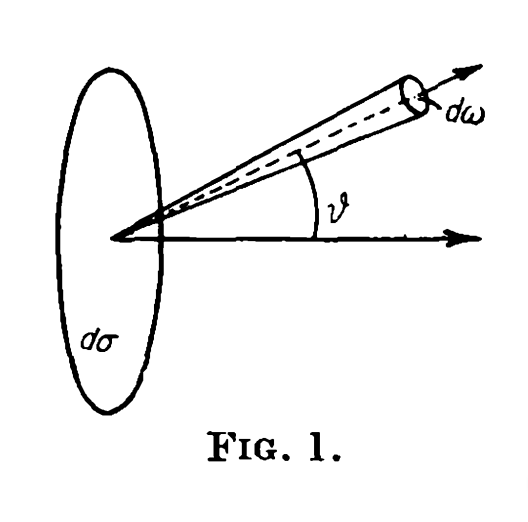
\includegraphics[width=0.3\textwidth]{fig/chandra.png}
    \caption{Figura del \textit{Radiative Transfer} de Chandrasekhar. }
    \label{fig:chandra}
\end{figure}
Nosotros suponemos que la radiancia de píxel está definida en función de un píxel observado, el cual tendrá una área $A_\px$, en la figura \ref{fig:chandra} sería $\diff\sigma$ integrado. El ángulo sólido $\diff\omega$ de la figura mencionada está relacionada al área de nuestro sensor $A_\sensor$, el cual está a una distancia $h_\LEO\approx 500$km de la superficie observada. El ángulo sólido entonces es
\[
\frac{A_\sensor}{h_\LEO^2}\qquad [\text{sr}]
\]


Se obtuvo el siguiente perfil (figura \ref{fig:ch4IrrVsPpm}) de radiancia de píxel ($\pixrad$) usando la herramienta 6S (Second Simulation of a Satellite Signal in the Solar Spectrum)

\simulationGraphic

Integrando la radiancia de píxel en longitud de onda se obtuvieron los siguientes valores (tabla \ref{tab:radianciasYModificada})

\begin{table}[htb!]
    \centering
    \begin{tabular}{lcc}
        \textbf{Caso} & \radiance [\radianceunits] & Atenuación [\%] \\ \hline
          \pixrad~ para 0ppm & 1.0858 & Referencia \\
          \pixrad~ para 3ppm & 1.0480 &  3.5\% \\
 %        \pixrad~ modificada & 1.0339 & 4.8\%
    \end{tabular}
    \caption{Radiancias para dos simulaciones de 6S y una simulación de 6S afectada por la transmitancia obtenida de Spectraplot. La atenuación va ser el valor medido para detectar presencia de \metano. Cabe destacar que la atenuación es casi lineal, 1\% caída en luz medida en el intervalo corresponde a 1ppm medido de \metano.}
    \label{tab:radianciasYModificada}
\end{table}


Luego se buscó estimar la corriente medida en el sensor (sección \ref{sec:senalRecibida}, \nameref{sec:senalRecibida})

\newpage
\section{Cálculo de señal recibida} \label{sec:senalRecibida}
Con la radiancia de píxel obtenida en la simulación se calcula la intensidad que llega al sensor según la altura del satélite $h_\LEO$ y el tamaño de píxel observado $A_\px$, el cual es el área observado sobre la tierra. 

\begin{equation}
    I_\sensor(\lambda) =  \frac{A_\px}{h_\LEO^2} \cdot  \pixrad(\lambda) \qquad [\text{W m}^{-2}\, \micro\text{m}^{-1} ] 
\end{equation}

El sensor ``convierte'' fotones a electrones. Nos interesa obtener el flujo de fotones sobre la superficie y según la longitud de onda. La energía de un fotón est\'a dada por $E_f = \frac{hc}{\lambda} $, por lo que dividimos por $E_f$ $[\text{W s fotón}^{-1}]$ 

\begin{equation}
    \Phi_\sensor(\lambda) = \frac{I_\sensor(\lambda)}{E_f} = \frac{I_\sensor(\lambda) \cdot \lambda }{hc} \qquad [\text{fotón m}^{-2}\, \micro \text{m}^{-1} \text{s}^{-1}] 
\end{equation}

Luego, multiplicando el valor $\Phi_\sensor$ por el área del sensor se obtiene la cantidad de fotones que inciden sobre el sensor por unidad de longitud de onda y por segundo. Para obtener la cantidad de electrones generados se integra la expresión obtenida multiplicada por la \textit{quantum efficieny} $Q$ del sensor $[\text{electrón foton}^{-1}]$, la cual también depende de la longitud de onda del fotón incidente, y luego se integra en el rango de longitudes de onda de interés.

\begin{equation}
    n_e = \int_{\lambda_1}^{\lambda_2} A_\sensor \cdot\Phi_\sensor(\lambda) Q(\lambda) \diff \lambda  \qquad [\text{electrón  s}^{-1}]
\end{equation}

La señal obtenida va a ser la corriente, que se obtiene multiplicando por la carga del electrón $q_e$ $[\text{coulomb electrón}^{-1}]$
\[
i_\sensor = n_e\cdot q_e \quad [\text{Amperes}] 
\]
Es necesario aún efectuar el análisis de \textit{signal to noise ratio} (S/N) partiendo del sensor elegido. A continuación se detalla un ejemplo del cálculo que se debería hacer suponiendo algunos valores:

\begin{itemize}
    \item Área de sensor (lente): $50$mm$^2$
    \item Área de píxel observado de 100km$^2$ (área de Manhattan)
    \item Variación de 1\% de la potencia recibida, que podría corresponder a una variación de 1ppm de \metano~ en la atmósfera según la tabla \ref{tab:radianciasYModificada}

    \item Quantum efficiency igual a 50\% constante
\end{itemize}



La corriente base que recibe el sensor es dado por 
\[
i_\sensor = n_e \cdot q_e = \frac{A_\sensor A_\px \cdot q_e}{h c (h_\LEO^2) } \cdot \int_{1,62}^{1.70} \lambda \cdot \pixrad(\lambda) Q(\lambda) \diff \lambda = 8.5363\times 10^{-8} \text{A}
\]

La corriente correspondiente a una variación de 1\% de \metano~ sería 
\[
\Delta i_\sensor = 1\% \cdot i_\sensor = 8.5363\times 10^{-10} \text{A}
\]

\section{Signal-to-noise Ratio (SNR)}

Para calcular el SNR se debe realizar el cociente entre en la señal medida con nuestro sensor y el ruido.\\
La señal del sensor se describe según la siguiente ecuación:

\begin{equation}
    \signal_\sensor = n_e \cdot q_e = \frac{A_\sensor A_\px \cdot q_e}{h c (h_\LEO^2) } \cdot \int_{1,62}^{1.70} \lambda \cdot \pixrad(\lambda) Q(\lambda) F_{MTF} T_p T_m \diff \lambda = XX\times 10^{-X} \text{A}
\end{equation}
siendo :
\begin{itemize}
    \item MTF= spreads light across multiple pixels ¿Aplica aquí??
    \item $T_m$: transmisividad, fracción de luz no absorbida. Tomada como constante $T_m=0.85$,
    \item Transparencia:
\end{itemize}

El ruido total \textit{N} se modela como un Ruido de Poisson, donde se considera que el ruido total es la raíz cuadrada de la suma de los cuadrados de los distintos ruidos que están presentes durante la medición, es decir:
\begin{equation}
   \noise=\sqrt{\sum_{i=1}^{n}\sigma_{i}^2}
\end{equation}

Donde los distintos ruidos involucrados en esta medición son: (REVISARLOS BIEN)\\


De esta manera el \textbf{SNR} queda expresado con la siguiente ecuación: (ARREGLARLA LUEGO DE REVISAR )

\begin{equation}
\mathrm{SNR}= \frac{\signal_\sensor}{\noise} =\frac{\frac{A_\sensor A_\px \cdot q_e}{h c (h_\LEO^2) } \cdot \int_{1,62}^{1.70} \lambda \cdot \pixrad(\lambda) Q(\lambda) F_{MTF} T_p T_m \diff \lambda}{\sqrt{\mathrm{F}^{2} \cdot \mathrm{G} \cdot\left(s_{\text {impact }}+s_{M}+s_{S L}+s_{D C}\right)+\sigma_{R O N}^{2}+\sigma_{O C N}^{2}+\sigma_{Q N}^{2}}}
\end{equation}

\end{document}

\[
\Delta i_\sensor = \Delta n_e \cdot q_e = \frac{A_\sensor A_\px \cdot q_e}{h c (h_\LEO)^2 } \cdot \int_{1,62}^{1.70} \lambda \cdot\Delta \pixrad(\lambda) Q(\lambda) \diff \lambda = 4.3826\times 10^{-10} \text{A}
\]
\todo[inline]{Para mi falta calcular la corriente base también, para mostrarla acá}
\todo[inline]{explicar cómo calculamos el delta}


\end{document}

\subsection{Cálculo de señal recibida}

Una vez obtenida la radiancia de píxel \pixrad~, se calcula la intensidad que llega al sensor según la altura del satélite $h_\LEO$ y el tamaño de píxel $A_\px$, el cual es el área observado sobre la tierra. 

\begin{equation}
    I_\sensor(\lambda) =  \frac{A_\px}{(R_\earth+h_\LEO)^2} \cdot  \pixrad(\lambda) \qquad [\text{W m}^{-2}\, \micro\text{m}^{-1} ] 
\end{equation}

El sensor convierte fotones a electrones. Nos interesa obtener el flujo de fotones sobre la superficie y según la longitud de onda. La energía de un fotón es dada por $E_f = \frac{hc}{\lambda}$ 

\begin{equation}
    \Phi_\sensor(\lambda) = \frac{I}{E_f} = \frac{I_\sensor(\lambda) \cdot \lambda }{hc} \qquad [\text{fotones m}^{-2}\, \micro \text{m}^{-1}] 
\end{equation}

Luego, multiplicando el valor $\Phi_\sensor$ por el área del sensor se obtiene la cantidad de fotones que inciden sobre el sensor. Para obtener la cantidad de electrones generados en corriente se integra la expresión obtenida multiplicada por la \gls{quantumeff} $Q$ del sensor, la cual también depende de la longitud de onda del fotón incidente.

\begin{equation}
    n_e = \int_{\lambda_1}^{\lambda_2} A_\sensor \cdot\Phi_\sensor(\lambda) Q(\lambda) \diff \lambda  \qquad [\text{electrones  s}^{-1}]
\end{equation}

La señal obtenida va ser la corriente, dada por
\[
i_\sensor = n_e\cdot q_e = n_e \cdot 1.602176634\times10^{-19} \qquad [\text{Amperes}]
\]
siendo $q_e$ la carga del electrón.
Es necesario aún efectuar el análisis de \textit{signal to noise ratio} (S/N) partiendo del sensor elegido. A continuación se detalla un ejemplo del cálculo que se debería hacer suponiendo algunos valores

\begin{itemize}
    \item Área de sensor $50$mm$^2$
    \item Área de pixel observado de 100km$^2$ (área de Manhattan)
    \item Variación de 1\% de la potencia recibida, que podría corresponder a una variación de 1ppm de \metano~ en la atmósfera según la tabla \ref{tab:radianciasYModificada}
    \item Quantum efficiency igual a 50\% constante
\end{itemize}

\[
\Delta i_\sensor = \Delta n_e \cdot q_e = \frac{A_\sensor A_\px \cdot q_e}{h c (R_\earth + h_\LEO)^2 } \cdot \int_{1,62}^{1.70} \lambda \cdot\Delta \pixrad(\lambda) Q(\lambda) \diff \lambda = 2.4\times 10^{-18} \text{A}
\]
La pregunta es contundente ¿como medimos esta corriente?

Formas de aumentar $\Delta i_\sensor$:
\begin{itemize}
    \item Acercarse lo más posible al rango de longitudes de onda donde el CH4 tiene más influencia (entre 1.665 y 1.6675)
    \item Aumentar $A_\px$, tener en cuenta la distancia focal.
    \item Aumentar $A_\sensor$, limitado por espacio disponible y lentes.
    \item Cambiar el modo de vibración observado a alguno que presente mayor absorbancia.
\end{itemize}{}

\bibliography{biblio}
%\addcontentsline{toc}{subsection}{\lstlistlistingname}

\end{document}